%%%%%%%%%%%%%%%%%%%%%%%%%%%%%%%%%%%%%%%%%%%%%%%%%%%%%%%%%%%%%%%%%%%%%
% Template for CSU thesis and dissertation submissions
%
% This template is compliant with the CSU formatting guidelines as of
% Fall 2017. Always send your thesis or dissertation to the library
% with plenty of time prior to the deadline for formatting feedback.
% No guarantees are made in regards to how well this template
% conforms to the current library standards.
%
%%%%%%%%%%%%%%%%%%%%%%%%%%%%%%%%%%%%%%%%%%%%%%%%%%%%%%%%%%%%%%%%%%%%%
% DocumentMetadata options
%%%%%%%%%%%%%%%%%%%%%%%%%%%%%%%%%%%%%%%%%%%%%%%%%%%%%%%%%%%%%%%%%%%%%
% DocumentMetadata is new to LaTeX. It increases accessibility and
% helps PDF files meet PDF standards. Note that uses these does not
% guarentee standard compliant PDF files. And, some features are still
% experimental and might not work with your files.
% The thesis class does not work with the following testphase options:
%    * block
%    * bib
%    * float
%    * math
% Given the list above, phase-III will not work until amsbook or
% DocumentMetadata is updated to address issues.
%
% References:
%   https://latex3.github.io/tagging-project/
%   https://mirrors.mit.edu/CTAN/macros/latex/required/latex-lab/documentmetadata-support-doc.pdf
%   https://mirrors.mit.edu/CTAN/macros/latex/required/latex-lab/latex-lab-table.pdf
% . https://latex3.github.io/tagging-project/tagging-status/
\DocumentMetadata
{
    lang = en-US,
    pdfversion = 2.0,
    pdfstandard = a-4f,
    pdfstandard = x-6,
    testphase ={
        phase-II,
        graphic,
        marginpar,
        minipage,
        sec,
        table,
        title,
        toc,
        firstaid,
    },
    xmp = true,
}
%%%%%%%%%%%%%%%%%%%%%%%%%%%%%%%%%%%%%%%%%%%%%%%%%%%%%%%%%%%%%%%%%%%%%
% Options for the documentclass
% -----------------------------
% masters
%   including 'masters' will change 'Doctor of Philosophy'
%   to 'Master of Science' for the degree
% 10pt, 11pt, 12pt
%   The title page, copyright page, and abstract are fixed at 12pt,
%   but you can change the body to one of three options
% times
%   Adobe Systems Utopia (1989) is the default serif font. Using
%   times will load newtxtext and newtxmath
% blue
%   makes the text for urls and references blue rather than black
%   requires the hyperref option
% smallfoot
%   makes the page number scriptsize rather than footnotesize
% nocopyright
%   CSU now requires the copyright page. If this changes, nocopyright
%   restores old format
%%%%%%%%%%%%%%%%%%%%%%%%%%%%%%%%%%%%%%%%%%%%%%%%%%%%%%%%%%%%%%%%%%%%%
\documentclass[masters,11pt,blue]{csuthesis}
%%%%%%%%%%%%%%%%%%%%%%%%%%%%%%%%%%%%%%%%%%%%%%%%%%%%%%%%%%%%%%%%%%%%%
% Title page
%%%%%%%%%%%%%%%%%%%%%%%%%%%%%%%%%%%%%%%%%%%%%%%%%%%%%%%%%%%%%%%%%%%%%
    \title{Epic title here}
    \author{John Doe}
    \departmentname{Atmospheric Science}
% Graduating term block
    \gradterm{Fall}
    \gradyear{2013}
% Committee block
    \advisor{Jane Doe}
    \coadvisor{John Doe} %optional
    \committee{Jane Doe \and John Doe \and Jane Doe}

\makeatletter

\begin{document}
%%%%%%%%%%%%%%%%%%%%%%%%%%%%%%%%%%%%%%%%%%%%%%%%%%%%%%%%%%%%%%%%%%%%%
% FRONT MATTER / PRELIMINARIES
%%%%%%%%%%%%%%%%%%%%%%%%%%%%%%%%%%%%%%%%%%%%%%%%%%%%%%%%%%%%%%%%%%%%%
\frontmatter
    \begin{abstract}
        \input{./pre/abstract.tex}
    \end{abstract}
    \begin{acknowledgments}     % optional
        The people you'd like to thank can go here.

    \end{acknowledgments}
    \begin{dedication}          % optional
        \begin{center}
\textit{People who put up with you can go here.}
\end{center}

    \end{dedication}
%%%%%%%%%%%%%%%%%%%%%%%%%%%%%%%%%%%%%%%%%%%%%%%%%%%%%%%%%%%%%%%%%%%%%
% Make Title Page and Table of Contents
%%%%%%%%%%%%%%%%%%%%%%%%%%%%%%%%%%%%%%%%%%%%%%%%%%%%%%%%%%%%%%%%%%%%%
\maketitle
\tableofcontents
\listoffigures   %optional
\listoftables    %optional
%%%%%%%%%%%%%%%%%%%%%%%%%%%%%%%%%%%%%%%%%%%%%%%%%%%%%%%%%%%%%%%%%%%%%
% CHAPTERS
%%%%%%%%%%%%%%%%%%%%%%%%%%%%%%%%%%%%%%%%%%%%%%%%%%%%%%%%%%%%%%%%%%%%%
\mainmatter
    \chapter{Introduction}
Epic introduction goes here.\\

Then you can do things like say as shown in Fig.\ \ref{fig:sample}
or add citations to epic papers like \cite{eliassen1951}. If we also decide
to add a table, we can add a reference to Table \ref{tab:lorenz}.

\begin{table}[t]
\caption[This caption appears in the LoT]{This is a sample table caption and
  table layout from the AMS LaTeX template file.Table from Lorenz (1963).}
\label{tab:lorenz}
\begin{center}
% Add tagging information to the table
% See documentation to understand how how this works.
% https://mirrors.mit.edu/CTAN/macros/latex/required/latex-lab/latex-lab-table.pdf
\tagpdfsetup{table-header-rows={1}}
\begin{tabular}{ccccrrcrc}
\hline\hline
$N$ & $X$ & $Y$ & $Z$\\
\hline
 0000 & 0000 & 0010 & 0000 \\
 0005 & 0004 & 0012 & 0000 \\
 0010 & 0009 & 0020 & 0000 \\
 0015 & 0016 & 0036 & 0002 \\
 0020 & 0030 & 0066 & 0007 \\
 0025 & 0054 & 0115 & 0024 \\
\hline
\end{tabular}
\end{center}
\end{table}

\begin{figure}[h!]
    \centering
    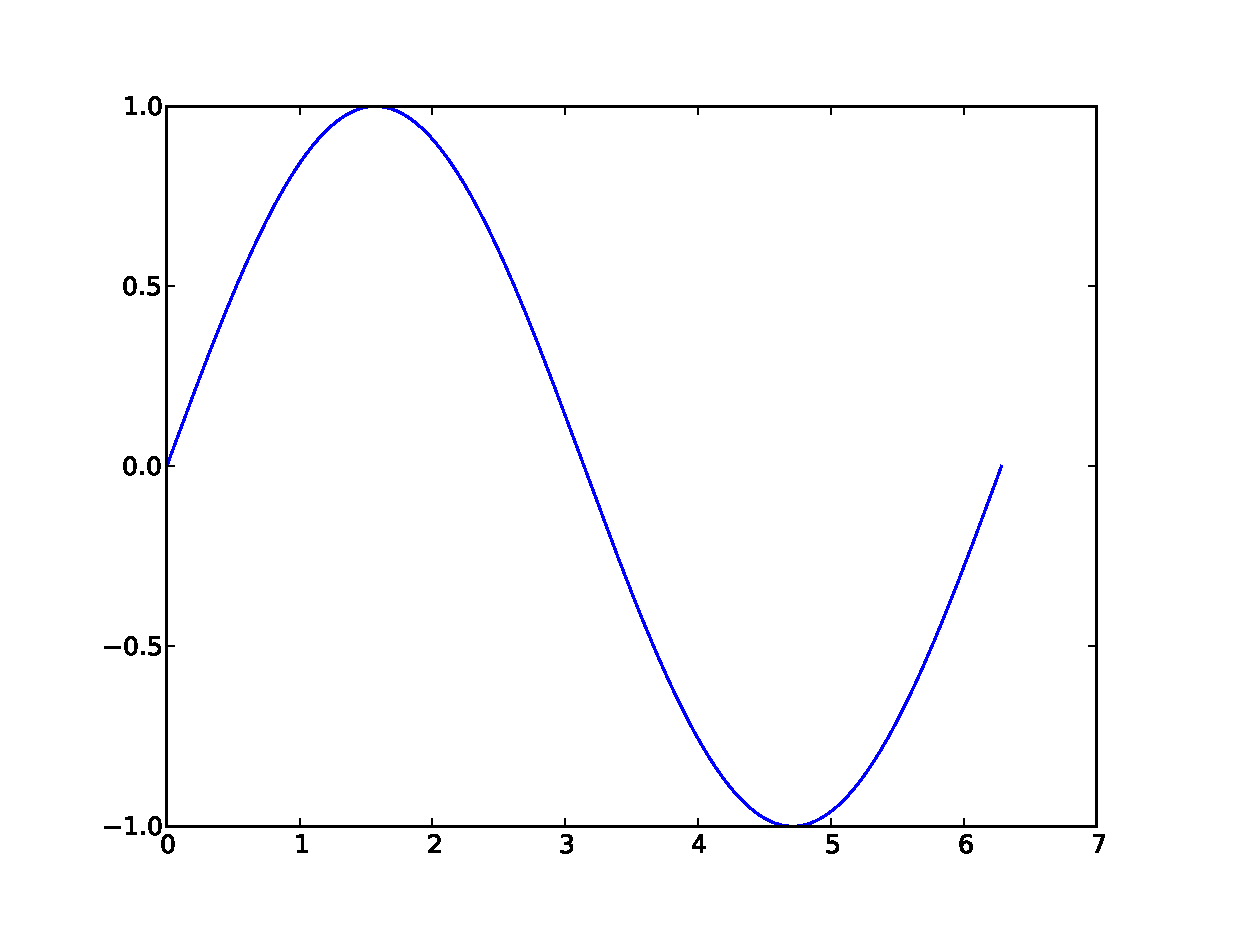
\includegraphics[width=0.75\textwidth,alt={This is alt text for a sine curve.}]{./chap1/fig/sample_fig}
    \caption[This caption is only in the LoF]{This is a sample figure with a
    sample caption.}
    \label{fig:sample}
\end{figure}

%%%%%%%%%%%%%%%%%%%%%%%%%%%%%%%%%%%%%%%%%%%%%%%%%%%%%%%%%%%%%%%%%%%%%
% REFERENCES
%%%%%%%%%%%%%%%%%%%%%%%%%%%%%%%%%%%%%%%%%%%%%%%%%%%%%%%%%%%%%%%%%%%%%
\backmatter
% Create a bibliography directory and place your .bib file there.
    {\clearpage}
    \bibliographystyle{ametsoc_csu}
    {\setstretch{1}
    \bibliography{references}}
%%%%%%%%%%%%%%%%%%%%%%%%%%%%%%%%%%%%%%%%%%%%%%%%%%%%%%%%%%%%%%%%%%%%%
% APPENDIX (optional)
% Use \appendix if there is only one appendix.
%\appendix
% Use \appendix[A], \appendix}[B], if you have multiple appendixes.
%\appendix[A]
%% Appendix title is necessary! For appendix title:
%\appendixtitle{}
%%%%%%%%%%%%%%%%%%%%%%%%%%%%%%%%%%%%%%%%%%%%%%%%%%%%%%%%%%%%%%%%%%%%%
    {\clearpage}
    \appendix
    \appendixtitle{Extra Stuff!}
    \section{Section of Extra Stuff}

\end{document}
